\section{Evaluation}
\label{sec:eval}

We conducted three different evaluations to show the effectiveness of our approach in
generating regression tests that achieve high code coverage. In our evaluations, we use
ten .NET base class libraries. Our empirical results show that our approach can generate
a high number of regression tests that can achieve a high code coverage. We next describe
the research questions addressed in our evaluation and present our evaluation results.

\begin{figure*}[t]
\centering
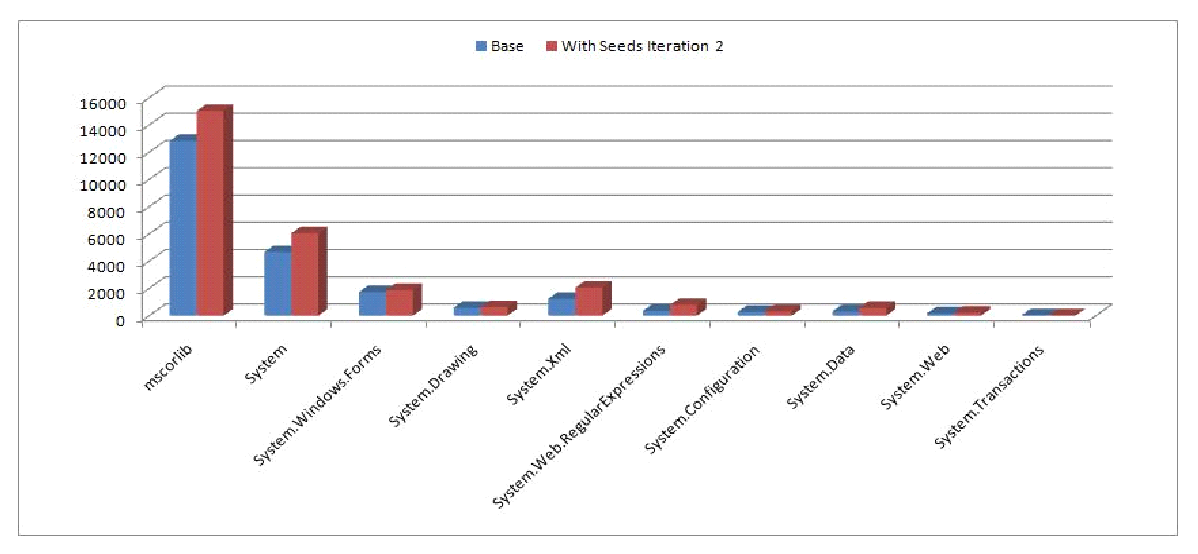
\includegraphics[scale=0.70,clip]{figs/RQ2_1.eps}\vspace*{-1ex}
\caption{Comparing code coverages achieved by base run and Run 4 (with seeds Iteration 2)} \label{fig:rq2}
\end{figure*}

%---------------------------------------------------------------------------------------
\subsection{Research Questions}
\label{sec:research}

We address the following three research questions in our evaluation.

\begin{itemize}
\item RQ1: Does our approach scale to a large number of PUTs? This research question helps
to show that our approach can address the scalability issues in dynamic symbolic execution.
\item RQ2: Do regression tests generated by our approach achieve higher code coverage? 
This research question helps to show the effectiveness of our approach in generating
regression tests that achieve a high code coverage.
\item RQ3: Do seed unit tests help achieve higher coverage than without using the tests?
This research question help to show that using existing unit tests as seed tests help
to achieve more code coverage than without using the tests.
\item RQ4: Does more machine power help achieve higher coverage? This research question
helps to address whether running the setup for more iterations help in achieving more coverage.
\end{itemize}

%---------------------------------------------------------------------------------------
\subsection{Subjects}

We used ten .NET base class libraries for evaluating our approach. Table~\ref{} shows
the ten libraries used in our evaluation and their statistics. TODO: Write more sentences
about the subjects here.

\setlength{\tabcolsep}{1pt}
\begin{table}[t]
\begin{SmallOut}
\begin{CodeOut}
\begin{center}
\begin {tabular} {|l|c|c|c|}
\hline
\textbf{.NET libraries} & \textbf{LOC} & \textbf{\# public} & \textbf{\# public}\\ 
 & & \textbf{classes} & \textbf{methods}\\ 
\hline
\hline  mscorlib & 185K & 1440 & 17800 \\
\hline  System &  & & \\
\hline  System.Windows.Forms & & & \\
\hline  System.Drawing & & & \\
\hline  System.Xml & 150K & 686 & 9920 \\
\hline  System.Web.RegularExpressions & & & \\
\hline  System.Configuration & & & \\
\hline  System.Data & 196K & 648 & 11550 \\
\hline  System.Web &  & & \\
\hline  System.Transactions & & & \\
\hline \textbf{AVERAGE} &  &  &   \\
\hline
\end{tabular}
\end{center}
\end{CodeOut}
\end{SmallOut}\vspace*{-4ex}
\centering \caption {Ten .NET base class libraries used in our evaluations}
\end{table}

%---------------------------------------------------------------------------------------
\subsection{Experimental Setup}

We next describe the experimental setup used in our evaluations. In our approach, we used nine 
machines that fall into three configuration categories. Table~\ref{} shows all three configuration
categories and the number of machines for each category used in our evaluations.

\setlength{\tabcolsep}{1pt}
\begin{table}[t]
\begin{SmallOut}
\begin{CodeOut}
\begin{center}
\begin {tabular} {|l|c|}
\hline
\textbf{Machine Configuration} & \textbf{\# of } \\  
 & \textbf{machines} \\  
\hline
\hline  Xeon 2 CPU @ 2.50 GHz, 8 cores, 16 GB RAM & 1 \\
\hline  Quad core 2 CPU @ 1.90 GHz, 8 cores, 8 GB RAM & 2 \\
\hline  Intel Xeon CPU @2.40 GHz, 1 GB RAM & 6 \\
\hline
\end{tabular}
\end{center}
\end{CodeOut}
\end{SmallOut}\vspace*{-4ex}
\centering \caption {Three categories of machine configurations used in our evaluations.}
\end{table}

In our evaluations, we used sandbox to restrict the access to external resources such
as files, registry, or unsafe code. We used this restriction to prevent the potential
corruption of the machines on which the tests are executed. Because of sandboxing,
the coverage achieved in our evaluations can be less than actual possible coverage
that can be achieved without using sandboxing. To address our research questions, 
we conducted four different runs. Each run took nearly two days. In Run 1, we ran
Pex to explore all PUTs once (Iteration 1) without using any seed unit tests.
In Run 2, we ran Pex for second iteration without using any seed unit tests. 
In Run 3, we used Pex to all explore all PUTs once (Iteration 1) with using 
seed unit tests. In Run 4, we used Pex for second iteration. We used the unit
tests generated from Iteration 1 as seed unit tests for Iteration 2.

%---------------------------------------------------------------------------------------
\subsection{RQ1: Scalability Issues}

We next address the first research question of whether our approach addresses scalability
issues in dynamic symbolic execution. In the capture phase, we recorded dynamic traces
of size $\approx$1.50 GB including 433,809 traces. The average trace length includes
$21$ method calls and the maximum trace length is $52$ method calls.
As capture phase transforms each dynamic trace into a PUT and a unit test 
(used as a seed test), the capture phase resulted in 433,809
PUTs and 433,809 unit tests. In the minimize phase, we filter out duplicate 
PUTs and unit tests. Our static analysis took 45 minutes to filter out 
duplicate PUTs. The number of minimized PUTs is 68,575. 

We used dynamic analysis to filter out duplicate unit tests. As it is not possible
to compile all 433,809 unit tests into a single project, we grouped these unit tests
into 943 projects based on the type under test in each unit test. Our dynamic analysis
took $\approx$5 hours and resulted in 128,185 minimized tests.

TODO: Shall we present an overview results of the number of tests generated here.

%---------------------------------------------------------------------------------------
\subsection{RQ2: High Code Coverage}

We next address the second research question of whether our approach generated 
regression tests that can achieve a high code coverage? To address this question,
we compare the code coverage achieved by unit tests generated from dynamic traces
(hereby referred as base coverage), and the coverage achieved by Run 4. We used
Run 4, as our approach achieved maximum coverage during Run 4.

Figure~\ref{fig:rq2} shows the results of comparing the base coverages with the coverages
achieved with Run 4 for all ten base class libraries used in our evaluation.
TODO: Describe about x-axis and y-axis. On average, our generated regression tests 
achieved 24.30\% higher coverage than the base coverage.

%---------------------------------------------------------------------------------------
\subsection{RQ3: Using Seed Tests}

We next address the third research question whether seed unit tests help achieve 
higher code coverage compared to without using seed tests. To address this question,
we compare the coverages achieved by Runs 2 (without seeds Iteration 2) and 4 (with seeds
Iteration 2). Figure~\ref{fig:rq3} shows the comparison of code coverages between these runs.
On average, using seed tests achieved 18.6\% more coverage than without using the tests.
TODO: To describe here the reasons why we are able to achieve higher coverage with seed tests.
TODO: Describe about x-axis and y-axis.

\begin{figure*}[t]
\centering
\includegraphics[scale=0.70,clip]{figs/RQ3_1.eps}\vspace*{-1ex}
\caption{Comparing code coverages achieved by base run, Runs 2 and 4 (with seeds Iteration 2)} \label{fig:rq3}
\end{figure*}

%---------------------------------------------------------------------------------------
\subsection{RQ4: Using More Machine Power}

We next address the fourth research question of whether more machine power helps to
achieve more coverage. To address this question, we show that later iterations achieve higher
coverages compared to previous iterations. For example, we show that Iteration 2 achieves 
more coverage compared to Iteration 1 for both scenarios of with and without using seed tests.

Figure~\ref{fig:rq41} shows the comparison of code coverages achieved by Runs 1 (without seeds Iteration 1) 
and 2 (without seeds Iteration 2). On average, Iteration 2 achieved 5.73\% higher coverage than 
Iteration 1. TODO: Describe about how it gets harder in going further.

Figure~\ref{fig:rq42} shows the comparison of code coverages achieved by Runs 3 (with seeds Iteration 1)
and 4 (with seeds Iteration 2). On average, Iteration 2 achieved 2.0\% higher coverage than
Iteration 1. TODO: Describe more about why with seeds has achieved less coverage compared to
without seeds between both the iterations.

\begin{figure*}[t]
\centering
\includegraphics[scale=0.70,clip]{figs/RQ4_1_1.eps}\vspace*{-1ex}
\caption{Comparing code coverages achieved by Runs 1 (without seeds Iteration 1) and 2 (without seeds Iteration 2).} \label{fig:rq41}
\end{figure*}


\begin{figure*}[t]
\centering
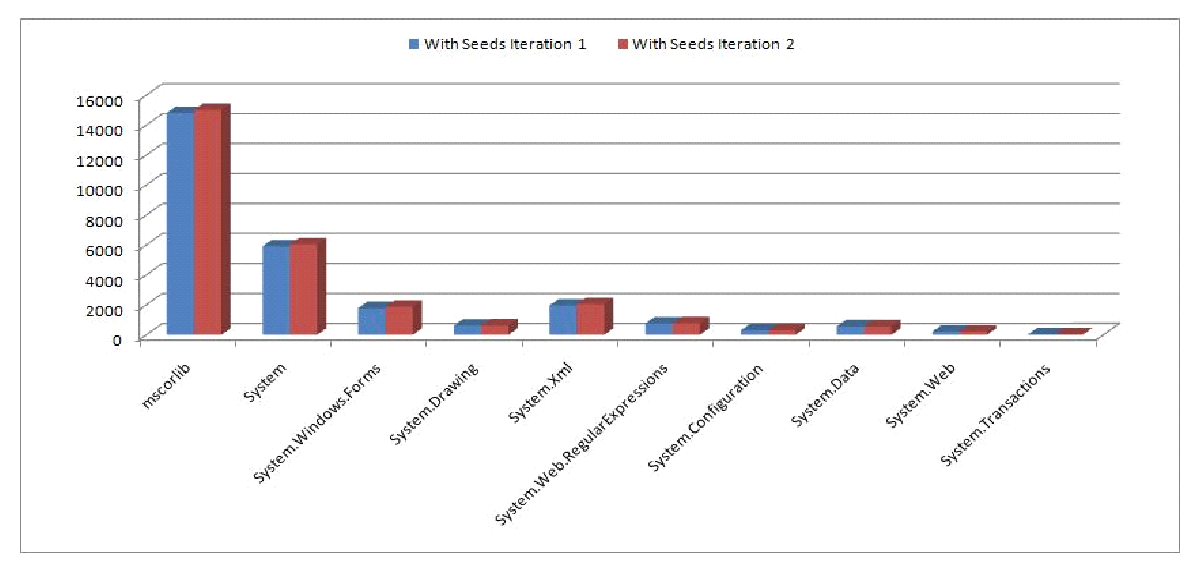
\includegraphics[scale=0.70,clip]{figs/RQ4_2_1.eps}\vspace*{-1ex}
\caption{Comparing code coverages achieved by Runs 3 (with seeds Iteration 1) and 4 (with seeds Iteration 2).} \label{fig:rq42}
\end{figure*}

%---------------------------------------------------------------------------------------
\subsection{Real Defects}

Our approach automatically generates test scenarios from dynamic traces. We use these test scenarios
in generating PUTs and then generating regression tests on a stable versions. These regression tests
can be used on future versions to detect regression faults. In our approach, we cannot detect
defects in the version on which regression tests generated because of lack of test oracles. However,
we identify that many exceptions are observed while generating regression tests on the version.
We next describe the raised exceptions and describe more about the defects detected.